%%%%%%%%%%%%%%%%%%%%%%%%%%%%%%%%%%%%%%%%%%%%%%%%%%%%%%%%%%%%%%%%%%%%%%%%%%%
%%%                                                                     %%%
%%%   LaTeX template voor het verslag van P&O: Computerwetenschappen.   %%%
%%%                                                                     %%%
%%%   Opties:                                                           %%%
%%%     tt      Tussentijdsverslag                                      %%%
%%%     eind    Eindverslag                                             %%%
%%%                                                                     %%%
%%%   3 oktober 2016                                   %%%
%%%   Versie 1.4                                                        %%%
%%%                                                                     %%%
%%%%%%%%%%%%%%%%%%%%%%%%%%%%%%%%%%%%%%%%%%%%%%%%%%%%%%%%%%%%%%%%%%%%%%%%%%%

\documentclass[tt]{penoverslag}
\usepackage{url}
\usepackage{amsmath}

%%% PACKAGES %%%



\begin{document}

% == TITELPAGINA == %
\team{Zilver}
\year{2016-2017}
\members{Bram Vandendriessche (Co\"ordinator)\\
         Arne Vlietinck (Secretaris)\\
         Matthias Van der Heyden \\
         Jef Versyck\\
         Vincent Vliegen\\
         Laura Vranken}
\maketitlepage


% == SAMENVATTING == %
\begin{abstract}
\noindent
{\em Auteur: Arne Vlietinck}\\
\\
Dit verslag behandelt het ontwerp en de implementatie van een Autopilot en Virtual Testbed voor een drone. In de simulator is voor de eerste mijlpaal een rode bol in een witte ruimte te zien. Bij de tweede mijlpaal wordt deze wereld uitgebreid met een windkracht in een willekeurige richting. Voor de derde mijlpaal zijn er verschillende bollen zichtbaar die allemaal op een zo efficiënt mogelijke manier moeten worden doorprikt. Bij de laatste mijlpaal zijn niet alle bollen direct zichtbaar. Een uitbreiding is het ontwijken van grijze obstakels.
\\
De Autopilot zorgt voor een correcte aansturing van de drone. Hij bepaalt de vliegroute op basis van informatie verkregen van twee camera's die zich op de drone bevinden. Hierbij is de relatieve plaatsbepaling van de bol ten opzichte van de drone van belang. De Autopilot leidt daaruit de beweging van de drone af en laat de simulator deze uitvoeren.
\\
Het programma wordt interactief gemaakt door het gebruik van \textit{GUI's}. Deze geven de mogelijkheid het camerastandpunt te kiezen, extra bollen toe te voegen, ook de voltooiingsgraad, snelheid en positie van de drone worden weergegeven. Daarnaast kunnen externe factoren (wind en gravitatieconstante) aangepast worden.


\end{abstract}


% == INHOUDSOPGAVE == %
\tableofcontents\newpage

%Dit zal dan verwijderd worden, wanneer het verslag volledig is.
%\em Enkele algemene richtlijnen : 
\begin{itemize}
\item Maak in het hele verslag gebruik van genummerde referenties, zoals hier ge\"\i llustreerd \cite{website:wikibooks-biblio}.  
\item Geef op het niveau van secties en/of subsecties aan wie de auteurs van dat deel zijn.  Een auteur is iemand die de tekst inhoudelijk en vormelijk mee bepaald heeft.    Als de secretaris of iemand anders de tekst vormelijk gewijzigd heeft, bv. om hem meer in lijn met de rest van het verslag te brengen, maar inhoudelijk niets toegevoegd heeft, is die persoon geen auteur maar een redacteur.  Je kan na de auteursnamen eventueel ``redactie: naam'' schrijven om aan te geven dat er substanti\"ele redactie gebeurd is (meer dan pakweg een paar tikfouten verbeteren).  Wanneer alle teamleden samen verantwoordelijk zijn voor een stuk (bv. samenvatting, conclusies) kan je de namen eventueel weglaten.
\item We verwachten dat alle groepsleden een substanti\"ele bijdrage leveren aan het  verslag, en dat dit ook zichtbaar is in de tekst!
\end{itemize}


\rm 

% == INLEIDING == %
\section{Inleiding}
\label{sec:Inleiding}
% \emph{[In de inleiding schets je de context, probleemstelling en doelstellingen van het project.  Je kunt ook kort aangeven wat er wel en niet in het verslag staat (bij een tussentijds verslag).]} 
{\em Auteurs: Laura Vranken \& Arne Vlietinck}
\\\\
\noindent
Drones zijn de laatste jaren enorm in populariteit toegenomen en blijven hierdoor ook in positieve zin evolueren. Ze worden tegenwoordig gebruikt voor talloze toepassingen. De bekendste toepassing bevindt zich binnen Defensie, die drones gebruiken om informatie te verkrijgen over vijandelijk gebied zonder mensenlevens te moeten riskeren. Daarnaast hebben ook grote bedrijven (o.a. Amazon\footnote{Amazon Prime Air}) de weg naar deze technologie gevonden. De toekomst brengt echter nog veel meer voordelen. Enkele voorbeelden  \cite{website:microdrones} zijn veiligheidsinspectie van windturbines of elektriciteitslijnen, luchtsteun bij zoek- en reddingsoperaties, bewaking en luchtfotografie.
\\
Wanneer een drone autonoom functioneert, is een betrouwbare aansturing door de Autopilot van levensbelang. Hij moet namelijk bestand zijn tegen allerlei externe factoren (bv. wind, obstakels...).
\\
\\
Dit verslag behandelt de autonome aansturing van een drone, meer bepaald een quadcopter, en is een vervolg op het tussentijds verslag \cite{arcticle:tssnTijds}. Er wordt uitgegaan van een drone waarop twee voorwaarts gerichte camera's bevestigd zijn. Op basis van deze beelden moeten afstand en positie tegenover het doel ingeschat worden en nieuwe bewegingsopdrachten voor de drone gegenereerd worden. Deze bewegingen worden weergegeven in een Virtual Testbed \cite{arcticle:opgavePeno}. Dit is een softwaresysteem dat een fysieke opstelling van een drone en camera's simuleert. De simulator genereert beelden van de drone uit verschillende standpunten a.d.h.v. de verkregen bewegingsopdrachten van de Autopilot. 
\\
\\
De Autopilot en Virtual Testbed moeten zo ontworpen worden dat de drone in staat is om zijn doel, een niet grijze bol, te lokaliseren en ernaar toe te vliegen. Dit eventueel onder lichte invloed van wind in willekeurige richtingen. Bovendien moet ook voor beiden een grafische user interface (\textit{GUI}) ontworpen worden. De \textit{GUI} toont de vooruitgang en laat de gebruiker toe allerlei informatie (snelheid, positie en verschillende camerastandpunten) op te vragen. Daarnaast kan de gebruiker nieuwe bollen toevoegen en de wind manueel aanpassen in de verschillende richtingen. 
\\
\\
De tekst is als volgt opgebouwd. %TODO


%Eerst wordt het ontwerp van de Autopilot en Virtual Testbed verder uitgediept (sectie \ref{sec:Ontwerp}). Vervolgens wordt er ingegaan op de gebruikte algoritmen (sectie \ref{sec:Algoritmes}) en wordt de opbouw van onze software verduidelijkt (sectie \ref{sec:Software}). Ook is er extra informatie te vinden over de \textit{GUI} (sectie \ref{sec:GUI}). Er wordt afgesloten met de uitgevoerde testen te bespreken (sectie \ref{sec:Testen}) en een kort besluit. \\


% == Beschrijving materiaal en bouw drone == %
\section{Ontwerp}
\label{sec:Ontwerp}
%[{\em Beschrijf het ontwerp van je softwaresysteem.  Schetsen of diagrammen kunnen hierbij nuttig zijn.  Bespreek je keuzes: vermeld alternatieven en motiveer je beslissingen.}]
\noindent {\em Auteurs: Arne Vlietinck; redactie: Arne Vlietinck}
\\
\\
\noindent
De concepten die gebruikt worden om het softwaresysteem te implementeren zijn van cruciaal belang. Hieronder wordt het stappenplan dat de Autopilot volgt, verduidelijkt en wiskundig toegelicht. Ook wordt er dieper ingegaan op de gemaakte keuzes tijdens de ontwerpfase. 





\subsection{Drone Autopilot}
{\em Auteur: Laura Vranken; redactie: Arne Vlietinck}\\

De Drone Autopilot zorgt voor de besturing van de drone. Het bepaalt zijn positie relatief ten opzichte van zijn doel aan de hand van twee beelden. Deze beelden zijn gemaakt door twee camera's die op de drone gemonteerd staan op een zekere afstand van elkaar. Bovendien kunnen ze opgevraagd worden vanuit de Virtual Testbed. Vervolgens zorgt de Autopilot ervoor dat de drone juist ge\"ori\"enteerd naar het doel staat en er naar toe vliegt. Wanneer de drone zijn doel,  een rode bol, bereikt, moet hij daarin blijven zweven. Tenslotte moet de Autopilot ook rekening houden met een mogelijke invloed van wind die de drone van zijn koers doet afwijken.\\

Ten eerste moeten dus de beelden die de Autopilot van de Virtual Testbed binnen krijgt, geanalyseerd worden. Dit gebeurt door iteratief de integer waarden van elke pixel te vergelijken met de waarde van de kleur rood. Alle rode pixels worden bijgehouden door hun positie ten opzichte van het beeld, uitgedrukt in rij en kolom, op te slagen. We baseren onze komende berekeningen op het midden van de bol. Dat midden kan bepaald worden door het zwaartepunt van de rode pixels te berekenen via het gemiddelde van de opgeslagen co\"ordinaten.\\

Indien de Autopilot geen rode pixels detecteert, zal de drone 360 graden ronddraaien of met andere woorden een yaw beweging uitvoeren, totdat in beide beelden rode pixels verschijnen. In het geval dat de Autopilot slechts rode pixels in een van de twee beelden opmerkt, zal het zichzelf door middel van een yaw beweging in de juiste richting bijsturen. Wanneer uiteindelijk in beide schermen rode pixels gevonden zijn, zal de Autopilot stoppen met draaien en zijn positie tegenover het doel berekenen.\\

Om zijn positie tegenover het doel te berekenen, bepalen we eerste de diepte. Dit kan met behulp van de formule van stereo vision (zie bron) uitgewerkt worden (en zie weergave in bijlage). Vervolgens bepalen we de hoek waaronder de drone een yaw beweging moet uitvoeren om recht naar het doel gericht te zijn. Deze formule kon afgeleid worden uit de goniometrie en wordt weergegeven in bijlage.. Om tenslotte naar het doel te kunnen vliegen, moet een evenwicht gevonden worden tussen pitch en thrust. De pitch hoek wordt gekozen zodat het zwaartepunt van het doel nog juist in beeld blijft. Die hoek is gelijk aan de helft van de verticale hoek die het beeld overspant min de verticale hoek waaronder de bol zich tegenover de drone bevindt (zie bijlage). Wanneer de pitch hoek vastligt, kan de hoeveelheid thrust berekend worden zodat de drone in rechte lijn naar het doel kan vliegen. (uitwerking formule)\\

Tenslotte moet dit proces herhaaldelijk worden uitgevoerd ten gevolge van de invloed van wind. De wind kan de drone namelijk uit koers brengen. Hierdoor zal de drone telkens zijn positie moeten herbepalen en zich opnieuw moeten herori\"enteren. Ook kan de wind ervoor zorgen dat de drone een roll uitvoert. Deze moet eerst gecompenseerd worden, vooraleer we verder onze berekeningen kunnen uitvoeren.\\

De drone bereikt zijn doel wanneer de Autopilot niks anders dan rode pixels opvangt. De drone zal dan de opdracht krijgen om zijn pitch te compenseren en vervolgens enkel via thrust de zwaartekracht tegen te werken. \\

Het effectief laten vliegen van de drone gebeurt in de Virtual Testbed waar de motoren worden aangestuurd. De Autopilot zendt enkel de verhouding in graden per seconden door waaronder pitch, yaw en roll moeten worden uitgevoerd en thrust in Newton. Het is slechts door herhaaldelijk te controleren hoe ver nog gedraaid moet worden, dat kan besloten worden wanneer de beweging volledig uitgevoerd is en wanneer gestopt mag worden.\\

Tegen de volgende deadline is het de bedoeling om de beeldverwerking via OpenCV uit te voeren. Deze bibliotheek kan op een betere en gemakkelijkere manier vormen en kleuren herkennen. Dit speelt in ons voordeel wanneer er meerdere doelen met verschillende vormen en kleuren in beeld zijn. Hierdoor vermijden we het iteratief zoeken en het moeten opslaan van pixels. Aangezien OpenCV op een bepaalde range in RGB waarden kan zoeken, kan ook het probleem van lichtinval en schaduw opgelost worden.
Ook wordt er gezocht naar een betere manier om de roll hoek in de berekeningen te trekken. Zo winnen we tijd aangezien die niet altijd eerst moet gecompenseerd worden voordat de berekeningen kunnen worden uitgevoerd. 


\subsection{Virtual Testbed}
{\em Auteur: Bram Vandendriessche}\\

%TODO!!

%TODO verwijzingen naar Blender, jmonkey en opengl toevoegen
\noindent
Voor de simulator is de belangrijkste keuze uiteraard welke library het meest geschikt is voor het bouwen, weergeven en aanpassen van 3D-werelden. Hiervoor werden Blender\footnote{\url{https://www.blender.org/}}, JMonkeyEngine\footnote{\url{http://jmonkeyengine.org/}} en OpenGL\footnote{\url{https://www.opengl.org/}} onder de loep genomen. 
\\
Blender is een erg uitgebreid programma met tal van mogelijkheden om 3D-objecten en -werelden te maken en manipuleren. Het maakt gebruik van Python, een programmeertaal met vrij eenvoudige leercurve voor wie al programmeerervaring heeft. Omdat we echter gepland hadden in Java te werken, moest gezocht worden naar een manier om Java en Python te verbinden. Bovendien zou Blender dan vanuit Java gestart moeten worden, wat een omslachtig proces bleek. Vooral omwille van de extra leertijd en deze laatste eigenschap werd niet voor Blender gekozen. \\
De tweede optie, JMonkeyEngine, leek erg gebruiksvriendelijk, met een goede tutorial en enkele handige ingebouwde functies, zoals het vastpinnen van een camera op een object. Helaas heeft deze \textit{API} een erg beperkte community waardoor problemen vaak zonder hulp van internet moeten worden opgelost. Ondanks de moeilijke beginfase bij het leren van OpenGL werd hiervoor gekozen. OpenGL kan rechtstreeks in Java worden gebruikt, heeft een tal van mogelijkheden en een brede community en er zijn heel wat tutorials beschikbaar. 

%TODO eventueel nog zeggen dat drone weergegeven wordt door balk, kan later nog aangepast worden

%Andere ontwerpkeuzes?


% == ALGORITMES == %
\section{Algoritmes}
\label{sec:Algoritmes}
%[{\em Beschrijf de algoritmes die je gebruikt.  Voor goed bekende of reeds bestaand algoritmes volstaat een verwijzing naar waar het algoritme beschreven staat.  Voor zelfgemaakte algoritmes is een duidelijke hoog-niveau beschrijving (bv. pseudocode) nodig.  Motiveer de keuze van algoritmes: welk probleem lost het algoritme op, waarom heb je dit algoritme gekozen en niet een ander?}]\\

\noindent {\em Auteurs: Jef Versyck; redactie: Arne Vlietinck}\\
\\
Om een realistisch beeld van de situatie te schetsen, is het belangrijk om op een juiste manier gebruik te maken van algoritmes. Ze be\"invloeden de correctheid en snelheid van het programma. Een verkeerde berekening kan immers leiden tot een waterval van andere fouten. Hieronder volgt een opsomming van alle gebruikte algoritmes in zowel de simulator als de Autopilot.


\subsection{Drone Autopilot}
\noindent {\em Auteurs: Laura Vranken }
\\
\\
De Autopilot gebruikt een algoritme om de hoeveelheid thrust te berekenen. De thrust wordt bepaald zodat de drone in een rechte lijn naar zijn doel vliegt. Zo vermijdt het onnodige bewegingen. Bovendien kan hierdoor ook de rode bol heel de tijd in beeld blijven. Een grafische voorstelling kan gevonden worden in figuur \ref{fig:GrafischeUitwerkingVanHoeveelheidThrustOnderBepaaldePitch}. Hierin is een drone onder een pitch \(\alpha\) voorgesteld, het zwaartepunt \(M\) van de rode bol staat relatief ten opzichte van de drone onder hoek \(\beta\) en zijn ook de drag \(D\), zwaartekracht \(F_z\) en thrust \(T\) voorgesteld.

\begin{figure}[h]
	\centering
	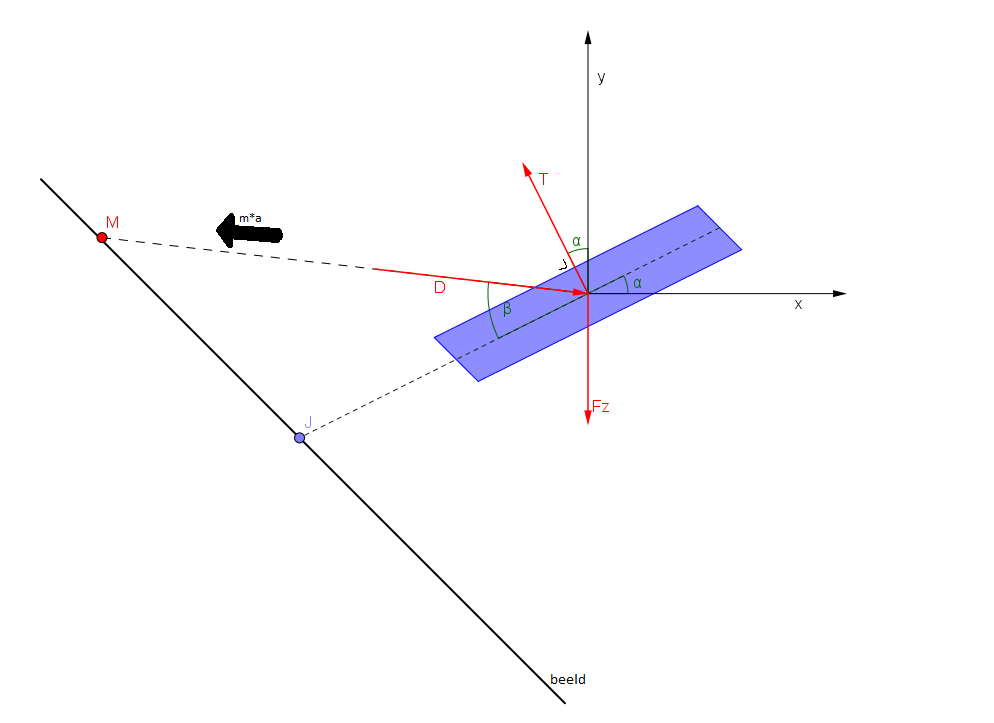
\includegraphics[width=0.5\textwidth]{GrafischeUitwerkingVanHoeveelheidThrustOnderBepaaldePitch.png}
	\caption{Grafische uitwerking van hoeveelheid thrust onder bepaalde pitch.}
	\label{fig:GrafischeUitwerkingVanHoeveelheidThrustOnderBepaaldePitch}
\end{figure}

\begin{equation}
\begin{cases}
T\cdot\sin(\alpha)-D\cdot\cos(\beta-\alpha) = m\cdot a\cdot\cos(\beta-\alpha)\\
T\cdot\cos(\alpha) - F_z - D\cdot\sin(\beta-\alpha) = m\cdot a\cdot\sin(\beta-\alpha)\\
\end{cases}
\end{equation}

\begin{equation}
\frac{T\cdot\sin(\alpha)-D\cdot\cos(\beta-\alpha)}{\cos(\beta-\alpha)} = \frac{T\cdot\cos(\alpha) - F_z - D\cdot\sin(\beta-\alpha)}{\sin(\beta-\alpha)}
\end{equation}

\begin{equation} \label{eq: thrustPitch}
T\cdot\sin(\alpha)\sin(\beta-\alpha) = T\cdot\cos(\alpha)\cos(\beta-\alpha)- F_z\cdot\cos(\beta-\alpha)
\end{equation}
Algemeen geldt er:
\begin{equation} \label{eq: gonio}
\cos(x+y) = \cos(x)\cos(y)-\sin(x)\sin(y)
\end{equation}
Door \ref{eq: gonio} toe te passen op vergelijking \ref{eq: thrustPitch} wordt volgende relatie afgeleid:
\begin{equation}
T = \frac{ F_z\cdot\cos(\beta-\alpha)}{\cos(\beta)}
\end{equation}




\subsection{Virtual Testbed}
\noindent {\em Auteurs: Jef Versyck}\\
\\
Het relatief assenstelsel hangt vast aan het centrum van de drone, zodat de linkercamera zich op de negatieve X-as bevindt en de rechtercamera op de positieve. De positieve Y-as staat loodrecht op de drone naar boven en de negatieve Z-as ligt in de diepte van het computerscherm. Het assenstelsel ondergaat identiek dezelfde bewegingen als de drone.
\\
\\
De drone kan drie bewegingen uitvoeren: roll, pitch en yaw. Het voert eerst zijn yaw uit, dan zijn roll en ten slotte zijn pitch. De yaw roteert rond de Y-as, de roll rond de Z'-as\footnote{Z-as van het relatieve assenstelsel na yaw beweging.} en de pitch rond de X''-as\footnote{X-as van het relatieve assenstelsel na alle vorige bewegingen.}. Merk op dat er een verschil bestaat tussen de roll en pitch die de drone op een gegeven ogenblik heeft en de yaw, roll en pitch die de drone moet uitvoeren om in zijn huidige positie te geraken. Daarnaast zijn door de ori\"entatie van het assenstelsel zowel de roll, pitch als yaw negatieve waarden.
\\
\\
Door de volgorde van de drie rotaties onstaat er een specifieke transformatiematrix die, vermenigvuldigd met de coördinaten van een punt (bv. het startpunt van de linkercamera), de coördinaten van het punt na de drie rotaties bepaalt. De verandering van de yaw/roll/pitch is ook afhankelijk van deze transformatiematrix. De verandering van de pitch is immers afhankelijk van de roll: hoe groter de roll, hoe trager de pitch verandert. 
\\
\\
De bekomen rotatiematrix:
\begin{equation*}
R = 
\begin{bmatrix}
\cos(Y)\cos(R) & -\cos(Y)\sin(R)\cos(P) + \sin(Y)\sin(P) & \cos(Y)\sin(R)\sin(P)+\sin(Y)\cos(P) \\
\sin(R) & \cos(R)\cos(P) & -\cos(R)\sin(P) \\ 
-\sin(Y)\cos(R) & \sin(Y)\sin(R)\cos(P)+\cos(Y)\sin(P) & -\sin(Y)\sin(R)\sin(P)+\cos(Y)\cos(P)\\
\end{bmatrix}
\end{equation*}
De berekening van de veranderingen van yaw, roll en pitch steunt op het principe
\begin{equation*}
R\textsuperscript{-1} \cdot R \cdot x = x
\end{equation*} 
met \(R\) de transformatiematrix, \(R\textsuperscript{-1}\) de inverse van de transformatiematrix en \(x\) de algemene beweging.  \(R \cdot x \)  is een relatieve beweging, zoals de verandering van de pitch. Deze relatieve beweging vermenigvuldigd met de inverse geeft de algemene beweging die de drone uitvoert voor die bepaalde verandering.
\\
\\
Elke drone heeft minstens twee krachten die erop uitgeoefend worden: de zwaartekracht en de thrust. De zwaartekracht is gelijk aan de massa maal de gravitatieconstante van de drone en zal altijd volgens de globale Y-as staan: \\
\begin{equation*} 
\vec{G} =
\begin{Bmatrix}
0 \\
m \cdot g \\
0 
\end{Bmatrix}.
\end{equation*} 
\\
De thrust \(T\) daarentegen is afhankelijk van de huidige pitch en roll van de drone. Daarom zal deze vermenigvuldigd moeten worden met de transformatiematrix, om de huidige thrust te bekomen. Het resultaat van deze vermenigvuldiging is: 
\begin{equation*} 
\vec{T} = 
\begin{Bmatrix}
T\cdot(\sin(P)\sin(Y) - \cos(P)\cos(Y)\sin(R))\\ 
T\cdot\cos(P)\cos(R) \\
T\cdot(\cos(Y)\sin(P) + \cos(P)\sin(R)\sin(Y))
\end{Bmatrix}.
\end{equation*}
\\
De windkracht, formule \ref{eq:windkracht}, is een kracht die een voorafbepaalde grootte en richting heeft. Deze kracht is optioneel in de implementatie. \\
\begin{figure}[h]
	\centering
	\begin{minipage}{.49\textwidth}
		\begin{equation}
		\vec{W} = 
		\begin{Bmatrix}
		W_x \\
		W_y \\
		W_z 
		\end{Bmatrix}
		\label{eq:windkracht}
		\end{equation}
	\end{minipage}
	\begin{minipage}{.49\textwidth}
		\begin{equation}
		\vec{F_d} = 
		\begin{Bmatrix}
		v_x \cdot d \\
		v_y \cdot d \\
		v_z \cdot d
		\end{Bmatrix}
		\label{eq:wrijvingskracht}
		\end{equation}
	\end{minipage}
\end{figure}
\\
De wrijvingskracht, formule \ref{eq:wrijvingskracht}, is een kracht die evenredig is met de snelheid \(v\) en een constante drag \(d\). Deze kracht werkt in tegen de snelheid, dus de constante is negatief.\\
\\
Alle vectorkrachten die inwerken op een bepaalde drone worden vervolgens bij elkaar opgeteld. Deze vector, gedeeld door de massa van de drone, zal gelijk zijn aan de versnelling van de drone, volgens de formule \ref{eq:somKrachten} \\
\\
Ten slotte kunnen via de snelheids- en positievergelijkingen de huidige snelheid en positie berekend worden. Respectievelijk formule \ref{eq:snelheid} en \ref{eq:positie}.
\begin{figure}[h]
	\centering
	\begin{minipage}{.49\textwidth}
		\begin{equation}
		\sum_{1}^{n} \vec{F_i} = m \cdot \vec{a} 
		\label{eq:somKrachten}
		\end{equation}
	\end{minipage}
	\begin{minipage}{.49\textwidth}
		\begin{gather}
		v = a\cdot t + v_0 \label{eq:snelheid}\\
		x = a\cdot \frac{t^{2}}{2} + v_0\cdot t + x_0 \label{eq:positie}
		\end{gather}
	\end{minipage}
\end{figure}




% == SOFTWARE == %
\section{Software}
\label{sec:Software}
%{\em Beschrijf het ontwerp van de software: klassediagrammen etc.}
\noindent {\em Auteurs: Arne Vlietinck; Redactie: Arne Vlietinck}
\\
\\
Tijdens het programmeren, is het belangrijk om een duidelijke structuur voor ogen te houden. Dit leidt immers tot goede leesbaarheid voor buitenstaanders en bewaart overzichtelijkheid bij lange code. Ook werd er geprogrammeerd met het doel om later gemakkelijk extra functionaliteiten te kunnen toevoegen.
\\
Om deze sectie beter te kunnen volgen, worden verschillende klassendiagramma's weergegeven in Appendix \ref{App: AppendixKlassendiagram}.


\subsection{Drone Autopilot}
\noindent {\em Auteur: Arne Vlietinck }
\\
\\
De aanmaak van een Autopilot en bijhorende \textit{GUI} gebeurt in de \textit{DroneAutopilotFactory}-klasse, ge\"implementeerd met de interface \textit{AutopilotFactory}. Hierin worden ook de beginwaarden voor yaw, roll, pitch en thrust direct ingesteld. 
\\
Door \textit{DroneAutopilotFactory} wordt een nieuw object \textit{DroneAutopilot} aangemaakt die de interface \textit{Autopilot} implementeert. De \textit{DroneAutopilot}-klasse bestaat uit één functie, namelijk \texttt{timeHasPassed()} die continu door de simulator wordt uitgevoerd. Vanuit deze methode wordt verwezen naar een bepaalde \textit{mission}-klasse die verder de opdracht voor zijn rekening neemt.
\\
\\
Er zijn twee missies die tot nu toe in de milestones nodig zijn namelijk \textit{OneSphere} en \textit{SeveralSpheres}. Hierdoor vliegt de drone respectievelijk naar een specifiek gekleurde bol of probeert hij alle bollen te bereiken. De keuze van de bepaalde missie wordt gemaakt in de \textit{GUI} door de gewenste missie te selecteren in het dropdownmenu. Om dit onderdeel aanpasbaar te maken, wordt een abstracte klasse \textit{Mission} voorzien, deze voorziet de basiselementen van de verschillende missies.
Elke missie selecteert op zijn beurt \textit{MoveToTarget} om de drone naar zijn beoogd doel te laten bewegen.
\\
\\
In \textit{MoveToTarget} worden de aansturing en bewegingen van de drone bepaald. Ook zullen de verschillende rates doorgegeven worden aan de simulator. Bovendien wordt hierin ook telkens de \textit{GUI} ge\"updatet wanneer een nieuwe waarde voor de diepte bepaald is.
\\
\\
Om de bewegingen te kunnen berekenen wordt er gesteund op twee \textit{calculation}-klassen namelijk \textit{ImageCalculations} en \textit{PhysicsCalculations}. Deze twee klassen staan los van de Autopilot, maar zijn van cruciaal belang om alles correct te laten verlopen. \textit{ImageCalculations} is verantwoordelijk voor alles omtrent de beelden die de Autopilot binnenkrijgt, m.a.w. de rode pixels zoeken en het zwaartepunt bepalen.
In de klasse \textit{PhysicsCalculations}, worden alle fysische berekening van hoeken en afstanden uitgevoerd.
\\
\\
Om de fouten die gemaakt zijn in de calculation-klassen binnen de perken te houden wordt zoals eerder al vermeld in sectie \ref{subsec: PI Controllers}, \textit{PI-controllers} voorzien. De algemene uitwerking van een controller wordt geïmplementeerd in een abstracte klasse \textit{PIController}. Voor elk te controleren waarde is er een specifieke controller. 
\\
Daarnaast wordt om de code van \textit{MoveToTarget} te verlichten \textit{Correctors} voorzien. In deze klassen wordt de methode gegeven hoe er moet omgegaan worden met de specifieke PI-controller. Terug is er een abstracte klasse voorzien om latere uitbreidingen gemakkelijker te maken. 
\\
\\



\subsection{Virtual Testbed}
{\em Auteur: Bram Vandendriessche}
\\

\noindent
Voor de simulator is geprobeerd om zo modulair mogelijk te werken, zodat nieuwe opstellingen of constraints gemakkelijk kunnen worden toegevoegd zonder dat dit voor problemen zou zorgen in de bestaande structuur. De klasse \textit{World} staat centraal in de simulator. Zij bevat alle basiselementen voor zowel het fysische als voor het 3D-gedeelte van de wereld. Het fysische aspect wordt behandeld door de klasse \textit{Physics}, wat al eerder werd besproken in sectie \ref{sec:AlgoritmesVirtualTestbed}. 
\\

\noindent
\textit{World} is ge\"implementeerd als een subklasse van \textit{GLCanvas} en legt de basis voor de 3D-weergave van de verschillende opstellingen. 
De klasse houdt bij welke \textit{WorldObjects} ze bevat (\textit{Spheres}, \textit{SimulationDrones}, \textit{ObstacleSpheres}) en implementeert enkele belangrijke functies voor de 3D-visualisatie ervan. De initialisatie van de wereld gebeurt door \texttt{init()}. De functie \texttt{draw()} roept de \texttt{draw()}-functie op van elk \textit{WorldObject} dat de wereld bevat. De \texttt{display()}-functie maakt meerdere keren gebruik van \texttt{draw()} om de wereld zowel naar het venster van de \textit{GUI} te renderen als naar de \textit{framebuffer objects} die dienen voor het offscreen renderen (voor \texttt{takeimage()}).\\
Bovendien bevat \textit{World} ook een abstracte methode \texttt{setup()}. Deze kan naar wens ge\"implementeerd worden door elke subklasse, zodat per mijlpaal een specifieke opstelling kan worden vastgelegd. Voor Milestone 1.1 is dit bijvoorbeeld enkel een rode bol, een drone en enkele camera's. Voor een wereld die vanuit een invoerbestand wordt opgebouwd met behulp van de parser, bestaat \textit{WorldParser}, waarbij de \texttt{setup()}-functie gebruik maakt van de geparste waarden.\\
\\
Uiteraard is er niets aan een 3D-wereld indien hij niet bekeken kan worden. De klasse \textit{GeneralCamera} werd ingevoerd om te kunnen werken met het concept van een camera, die een positie en kijkrichting krijgt. Zulke camera's kunnen dan op verschillende punten geplaatst worden (vastgelegd in de \texttt{setup()} van de wereld), zodat de gebruiker de voortgang van de drone goed kan volgen. Een uitbreiding op dit concept is de \textit{DroneCamera}, die zich voor zijn positie en ori\"entatie op de drone (waartoe hij behoort) zal baseren. Dit laatste type kan gebruikt worden voor de ``ogen'' van de drone en deze klasse implementeert de \textit{Camera}-interface van de \textit{API} voor de verbinding van Autopilot en Testbed.\\
Deze rol vult \textit{SimulationDrone} in voor de \textit{Drone}-interface. Deze klasse tekent de drone als een blauwe balk.




% == GUI == %
\section{GUI}
\label{sec:GUI}

\noindent {\em Auteurs: ; redactie: Arne Vlietinck}\\

%{\em Beschrijf het ontwerp van de GUI in termen van lay-out, gebruik, interactie, \ldots}


\subsection{Drone Autopilot}
\noindent {\em Auteur: Matthias Van der Heyden}\\
De GUI van de drone autopilot heeft tot nu toe twee functies: de gebruiker de mogelijk geven een opdracht voor de drone te selecteren en de voortgang van de voltooiing van deze opdracht weergeven.
Voor de layout van de GUI wordt Java's Abstract Window Toolkit (java.awt) gebruikt.\\

Voor het selecteren van een opdracht is er een drop-down menu voorzien dat gebruikt maakt van JComboBox uit de Swing library van Java. Wanneer de gebruiker een optie aanduidt, verandert de boolean van deze optie naar true. Dat zorgt er voor dat in de timeHasPassed functie de commando's voor deze opdracht uitgevoerd worden. Op dit moment is de enige optie in het menu de opdracht om naar de rode bol te vliegen maar een uitbreiding van mogelijke opdrachten is relatief eenvoudig.\\

Een JProgressBar uit de Swing library van Java geeft in de GUI de voltooiing van de geselecteerde opdracht weer. Bij elke berekening van de afstand tot het doel wordt deze ge\"{u}pdatet. Is de afstand groter dan de laatste grootste afstand tot het doel dan stelt de progress bar deze nieuwe afstand in als het nieuwe maximum en is de voltooiingsgraad weer 0. Is de afstand kleiner dan is de nieuwe voltooiingsgraad gelijk aan 100 procent vermindert met de verhouding van de grootste afstand en de huidige afstand.  



\subsection{Virtual Testbed}
\noindent {\em Auteurs: Arne Vlietinck}
\\
\\
In het Virtual Testbed wordt een panel van vaste grootte voorzien waarin de \textit{GUI} vervat zit. In tegenstelling tot de Autopilot wordt hier gebruik gemaakt van een iets uitgebreidere lay-outvorm namelijk de \textit{GridBagLayout}\footnote{\textit{GridBagLayout}: https://docs.oracle.com/javase/7/docs/api/java/awt/GridBagLayout.html}. Dit zorgt voor een op maat gemaakte lay-out, die noodzakelijk was voor het uitlijnen van de verschillende functies. 
\\
\\
De centrale functie van deze \textit{GUI} is het selecteren van verschillende camerastandpunten. Dit kan door middel van de opties in het dropdownmenu of via \textit{JButtons}. Naargelang de hoeveelheid camerastandpunten zullen er automatisch extra opties in het menu gegenereerd worden. De basiscamera's bestaan uit de verschillende wereldcamera's, de linkerdronecamera en een third-personcamera, die de drone op de voet volgt. Naast deze verschillende opties kan er in het scherm van de wereldcamera gebruik gemaakt worden van de pijltjestoetsen (en P\&M) \footnote{Respectievelijk links, rechts, voorwaarts en achterwaarts met de pijltjestoetsen en opwaarts (P) of neerwaarts (M).} om de drone naar wens te volgen. 
\\
\\
Naast de mogelijkheid om de camera's te kiezen, worden er ook \textit{JSliders} voorzien die het mogelijk maken de wind (in \(x\)-, \(y\)- en \(z\)-richting) en gravitatieconstante aan te passen naar behoeven. Zo kan ten allen tijde de invloed van respectievelijk de wind en zwaartekracht onderzocht worden. Wanneer er gewerkt wordt met de \textit{WorldParser} zijn er reeds windkarakteristieken meegegeven. Indien dit het geval is, zal er enkel een output zijn van de windsterkte in verschillende richtingen.
\\
Ook wordt de snelheid en de positie van de drone weergegeven. Deze wordt continu opnieuw opgevraagd en ge\"{u}pdatet in de \textit{GUI}. 
\\
\\
Tot slot wordt er nog een button voorzien waarmee het mogelijk is om een nieuwe bol toe te voegen. Door de button te gebruiken, opent er een nieuw frame waarin de gewenste co\"ordinaten ingegeven kunnen worden. 


% == Testen == %
\section{Testen}
\label{sec:Testen}
%[{\em Beschrijf de tests die je uitgevoerd hebt om de correcte werking en de nauwkeurigheid van je software te bepalen.  Geef de resultaten op compacte en heldere manier weer, bv. met tabellen of grafieken.  Denk na over de beste manier om de resultaten weer te geven.  Ze moeten je conclusies ondersteunen.  Formuleer de conclusies.}]\\

\noindent {\em Auteurs: Arne Vlietinck; redactie: Arne Vlietinck}
\\
\\
Voor beide programma's worden er uitvoerig testklasses gegenereerd en uitgevoerd. Hiermee kan de correcte werking en de nauwkeurigheid van de gebruikte algoritmes gecontroleerd worden. Ook eventuele programmeerfouten komen aan het licht en kunnen op deze manier aangepast worden. 
\\
Naar gelang de milestones uitdagender worden, zullen de testklassen striktere en hogere eisen stellen aan de ge\"implementeerde tests.


\subsection{Drone Autopilot}
\noindent {\em Auteurs: Vincent Vliegen}\\

De autopilot is voorzien van enkele JUnit testclasses. Deze testen de verschillende gebruikte methods op hun nauwkeurigheid en correctheid. Zo is het eenvoudiger de capaciteiten van de autopilot aan te tonen en de beperkingen duidelijk af te bakenen.

De ImageCalculationsTest is uitgerust met tests voor elke method in de ImageCalculations class. Er is gebruik gemaakt van een anonieme class die de Camera interface implementeert, opdat er afbeeldingen naar keuze gegenereerd kunnen worden, die het testen praktisch vereenvoudigen.

De PhysicsCalculationsTest verschaft testmethodes voor de PhysicsCalculations class. Ook hier zijn anonieme classes ge\"implementeerd, namelijk voor de Camera en Drone interfaces.

% MoveToTargetTest nog niet uitgewerkt, geen test voor droneautopilot(factory)
%zou ik verdere/betere uitleg geven over de anonieme classes?


\subsection{Virtual Testbed}
\noindent {\em Auteur: Jef Versyck}
\\
\\
Het testen van bepaalde functies van de simulator gebeurt via een aangemaakte \(dummy\) wereld die enkel een \textit{SimulationDrone}, een \textit{Sphere} en een \textit{ObstacleSphere} bevat. Om de collision detection te testen, worden beide \textit{Spheres} eerst apart, vervolgens tesamen op de drone geplaatst en wordt telkens collision detection opgeroepen. Ten tweede wordt de bol net buiten en net binnen het verwachte bereik geplaatst en wordt wederom collision detection opgeroepen. 
%Voor het testen van de slaagkansen van de Autopilot op de milestones, werd meerdere keren de simulatie gerunt op verschillende testwerelden. De resultaten hiervan bevinden zich in de bijlagen.



% == ... == %
\section{\ldots}


% == BESLUIT == %
\section{Besluit}
\label{sec:Besluit}
\noindent {\em Auteurs: Arne Vlietinck; redactie: Arne Vlietinck}
\\
\\
Dit verslag rapporteert het cre\"eren van een drone Virtual Testbed en zijn Autopilot. De Autopilot berekent de juiste instructies a.d.h.v. de dronecamera's. Via deze beelden slaagt de Autopilot erin om de drone de eerste bol te laten doorprikken. Van groot belang om dit geheel te laten werken, is een juiste visualisatie door de simulator. Daarnaast moeten alle bewegingen in juist volgorde uitgevoerd worden op zowel de drone als camera's. Zoals er beschreven staat in de mijlpalen werd er ook een variabele windfactor ge\"implementeerd. Wanneer de wind van toepassing is, is het halen van de mijlpalen niet altijd mogelijk. 
\\ 
Daarnaast worden de vele keuzes die tijdens het project gemaakt werden, verdedigd in bovenstaande secties.
\\
Tijdens het programmeren werd een duidelijk schema voor ogen gehouden zodanig dat uitbreidingen voor eventueel volgende mijlpalen vlot kan verlopen.\\

% == REFERENTIES == %
\bibliographystyle{siam}
\bibliography{references.bib}


% == APPENDICES == %
\newpage\makeappendix

\section{Klassendiagram Autopilot} \label{App:KlassendiagramAutopilot}

\begin{figure}[h]
	\begin{center}
		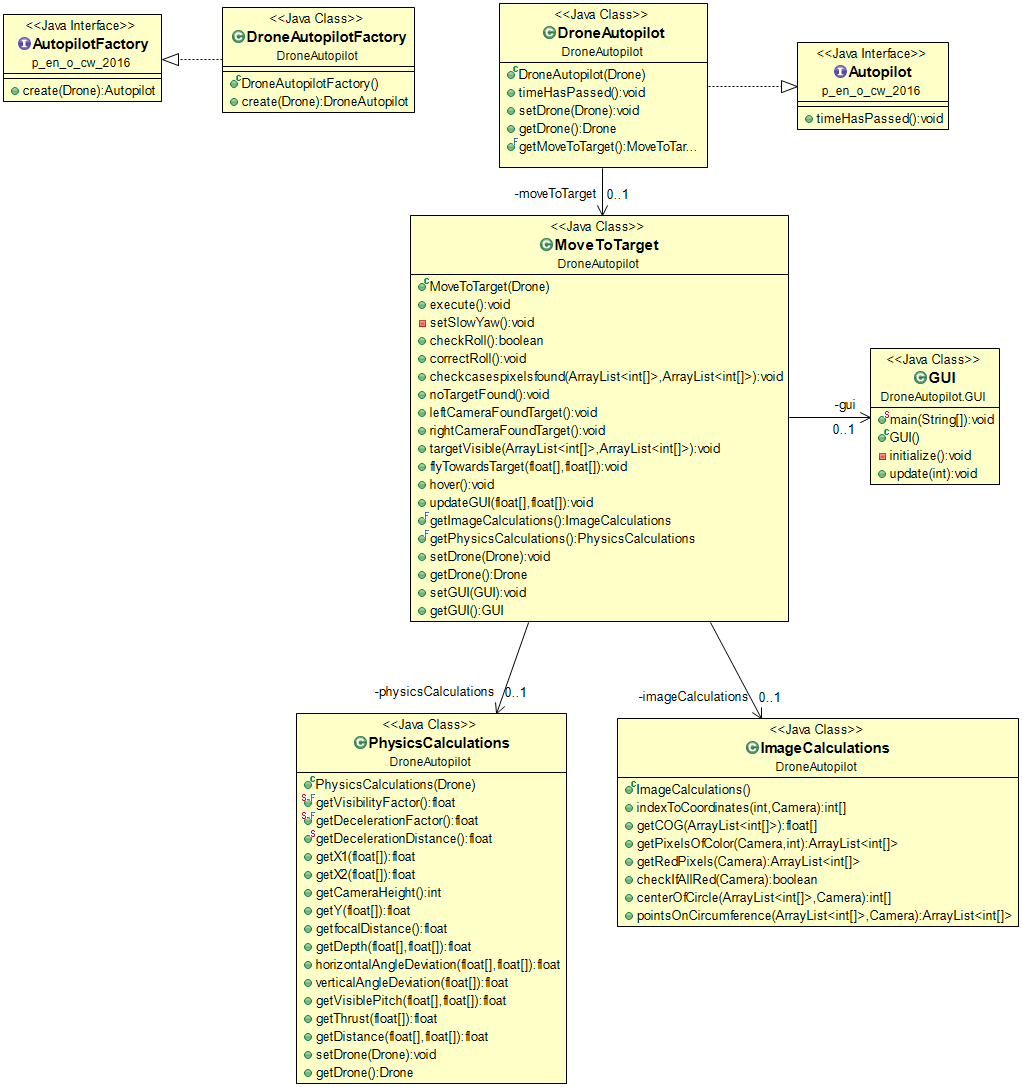
\includegraphics[width=\textwidth]{KlassendiagramAutopilot.png}
	\end{center}
\end{figure}

\section{Klassendiagram Simulator} \label{App:KlassendiagramSimulator}

\begin{figure}[h]
	\begin{center}
		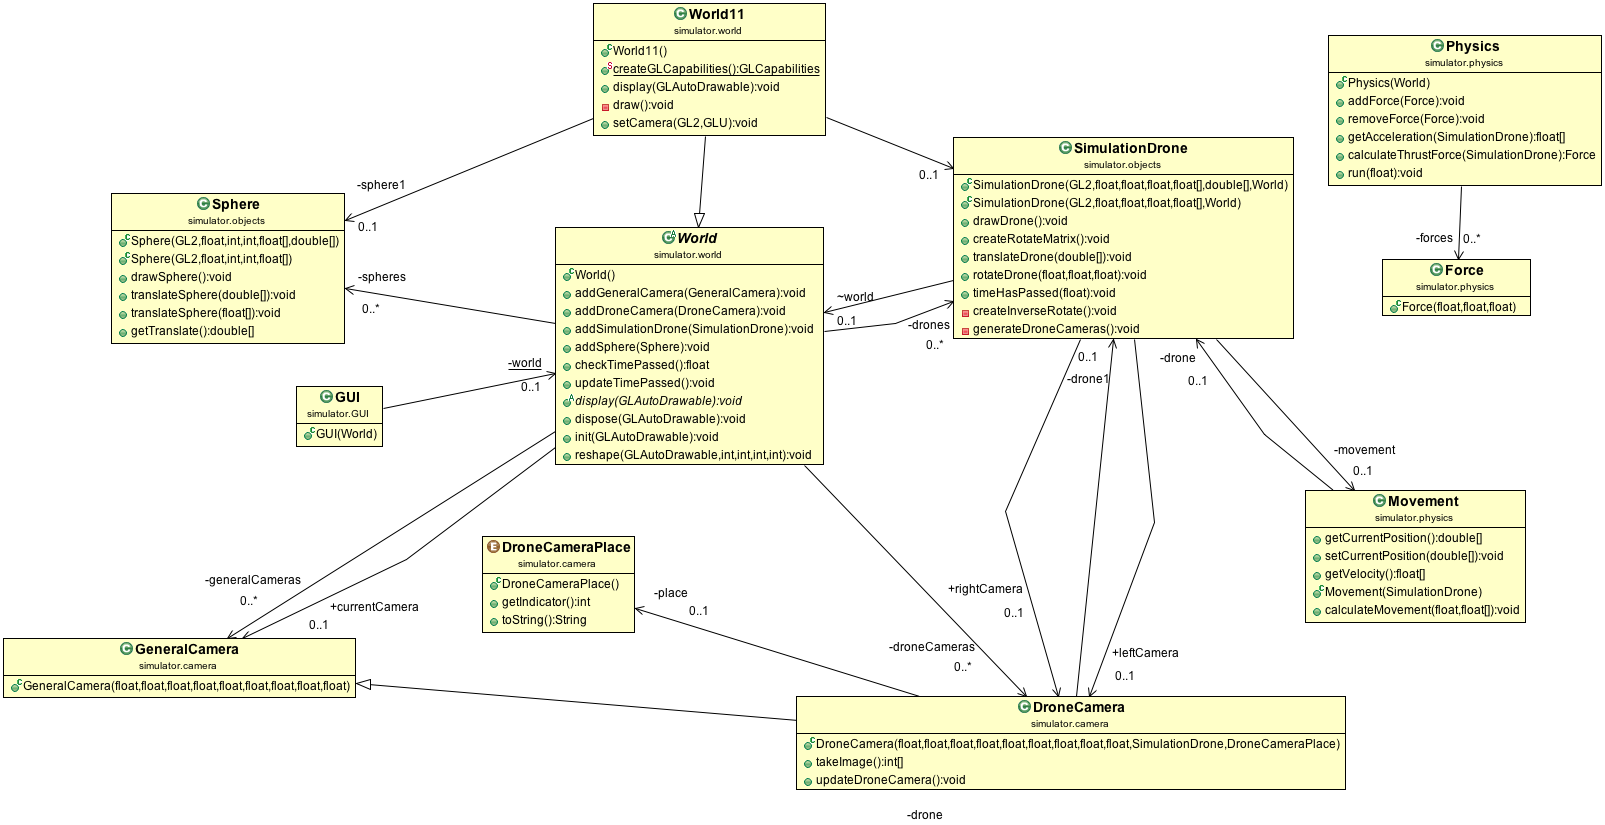
\includegraphics[width=\textwidth]{KlassendiagramSimulator.png}
	\end{center}
\end{figure}

\section{MOET NOG WEG}
De volgende informatie wordt na de finale demonstratie apart ingediend.

\section{Beschrijving van het proces}
\begin{itemize}
\item Welke moeilijkheden heb je ondervonden tijdens de uitwerking?
\item Welke lessen heb je getrokken uit de manier waarop je het project hebt aangepakt?
\item Hoe verliep het werken in team? Op welke manier werd de teamco\"ordinatie en planning aangepakt?
\end{itemize}


\section{Beschrijving van de werkverdeling}
\begin{itemize}
\item Geef voor elk van de groepsleden aan aan welke delen ze hebben meegewerkt en welke andere taken ze op zich hebben genomen.
\item Rapporteer in tabelvorm hoeveel uur elk groepslid elke week aan het project gewerkt heeft, zowel tijdens als buiten de begeleide sessies. Geef ook totalen per groepslid voor het volledige semester.
\end{itemize}


\section{Kritische analyse}
\begin{itemize}
\item Maak een analyse van de sterke en zwakke punten van het project. Welke punten zijn vatbaar voor verbetering. Wat zou je, met je huidige kennis, anders aangepakt hebben?
\end{itemize}



\end{document}
